\chapter{Impact of Human specific variants on modern human biology}
\section{Introduction}
Uncovering genetic changes that make anatomically modern humans “unique” is critical for a comprehensive understanding of human evolution. Recent genomic advantages have began to elucidate the nuances of human evolution and how humankind relates to some of our closest hominid relatives. These advances are starting to reveal how intermixing between species has shaped modern human biology. Research has been done examining how regions of DNA that have been passed into homosapiens from our closest relatives, suggesting that some of this introgressed DNA may be adaptively beneficial or undergoing negative selection. On the other hand, there have been studies showing variant regions of DNA that are human-specific, or lacking in our closest relatives, suggesting that these mutations may have been important in developing modern human biology. Some studies show (**add examples, foxp2,etc).
By analyzing genome sequences from our closest evolutionary relatives, Neanderthals and Denisovans, we can functionally characterize these genetic changes. Towards this end, we identified 50,505 mutations that are nearly fixed for the derived allele in African individuals from the 1000 Genomes project ($>90\%$ derived allele frequency) but are absent in all of the deeply sequenced Altai and Vindija Neanderthal and Denisovan genomes. Here we look at some of these human specific regions and how they impact modern human phenotypes.

To understand the phenotypic impact of these fixed derived mutations (FDMs), we leverage the observation that interbreeding with Neanderthals likely re-introduced the ancestral allele at a number of these sites. We estimate that $~39\%$ of FDMs are polymorphic in European populations so that their phenotypic impact can be analyzed by genotyping these mutations in large cohorts with phenotypic information.These Fixed Derived alleles (FDs) are mutations that rise to high frequency  in  modern  humans  since  the  split  from  archaic humans, and may give us clues to the biology that cause modern humans to differ from our closest relatives.
\section{Results}
\subsection{Identifying genomic regions at which fixed derived mutations influence phenotypes}
To understand how human specific mutations influence trait variation we first annotated the fixed derived mutations in the UK biobank. One approach we can use is to look at genetic components of traits that modern humans share, and our archaic relatives, such as the Neanderthal, don’t. In other words, we wanted to identify derived mutations in the modern human genome that differed from our ancient relatives, and rose to high frequency. These mutations occur after modern humans split from Archaic individuals such as Neanderthals, and then rise to a high frequency in modern humans. In order to overcome the problem of these mutations becoming fixed, or at nearly 100 \% allele frequency, we leverage the fact that introgression may have reintroduced variation into these mutations in European individuals (Fig 1). We first identified 50,505 (25,448) mutations that were $>99\% (>95\%)$ for the derived allele in 1000 genomes phase 3 African populations and ancestral in the Altai Neanderthal or Denisovan and deemed Fixed Derived mutations. These mutations are heterozygous in a number of White British individuals in the UK Biobank (Fig 2 & 3). After identifying the $FDMs >99\%$, we used plink2 to run GLM on 96 phenotypes to find 464 FDMs associated with 39 phenotypes at a p-value threshold of $p<10^{-10}$. After clumping analysis we find 70 independent associations of the 39 phenotypes.
\section{Methods}
\subsection{Cohort}
\subsection{Identifying Fixed Derived Mutations}
 We first determined derived allele frequencies from African individuals in the 1000 genomes project phase3. We combined allele frequencies from ESN, GWD, LWK, MSL, YRI individuals in 1000 genomes in order to determine an African derived allele frequency (. We then determine the allele frequency in archaic individuals combining Vindija, and Altai neanderthals as well as the Denisovan individual. Combining the datasets, we examined 41,864,101 SNPs. We then filtered out SNPs with an African derived allele frequency >0.95 and >0.99 to find 50,505 and 25,448 mutations that are likely human specific. We then intersected these variants with those in the UK Biobank to find 19,632 and 9,407 fixed derived mutations able to be tested.
\subsection{UK Biobank (UKBB) genotype QC}
We restricted all our analyses to a set of high-quality imputed SNPs (with a hard call threshold of 0.2 and an info score greater than or equal to 0.8), which, among the 291,273 imputed genotypes of UKBB unrelated white British individuals, 1) have MAF higher than 0.001, 2) are under Hardy-Weinberg equilibrium ($p > 10^{-7}$), and 3) are confidently imputed in more than 99\% of the genomes. Additionally, we excluded SNPs in the MHC region, resulting in a total of 7,774,235 SNP which we refer to as QC-ed SNPs. 
\subsection{Association Testing}
To identify individual FDMs associated with a phenotype, we fit a linear regression model using plink 2.0 --glm and included covariates controlling for age, sex and the first 20 genotypic PCs, and first five FDM PCs. We used a stringent p-value threshold of $10^{-10}$ to correct for the number of FDMs and phenotypes tested. For each phenotype, we clumped all significant NIMs that lie within 250 kb and with an LD threshold ($r^2$) of 0.5 using a significance threshold for the index SNP of $10^{-10}$.

\section{Figures}
\begin{figure}[htb]
    \centering
    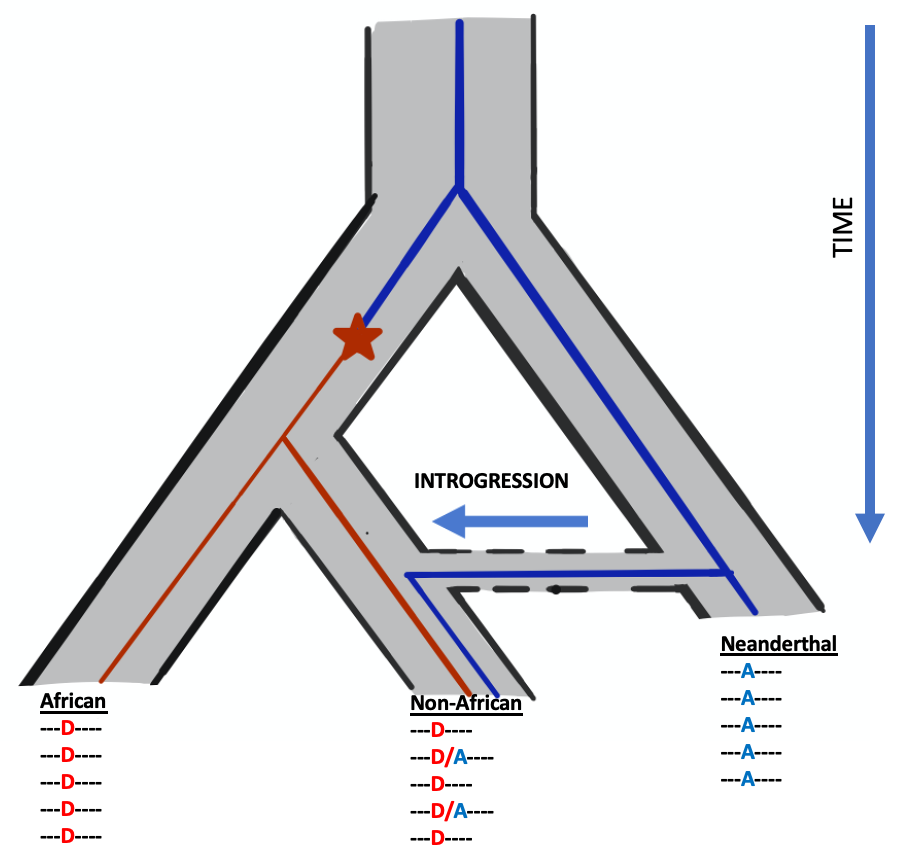
\includegraphics{chapter4/figures/fig41.png}
    \caption{Caption}
    \label{fig:my_label}
\end{figure}
